\chapter{Results and Discussion}

\section{Model Parameters}

Using the $70\%$ training set, $15\%$ validation set, and $15\%$ testing set, the hyperparameters chosen for each learning model is shown in \cref{tab:hyperparam}.

\begin{table}[h]
	\centering
	\caption{Final hyperparameters for learning models}
	\label{tab:hyperparam}
	\begin{tabular}{@{}ll}
		\toprule
		Model                & Parameters                                                                                    \\ \midrule
		Ridge Regression     & $\lambda=10$                                                                                  \\
		Huber Regression     & $\epsilon = 1.0$                                                                              \\
		                     & $\alpha=0.001$                                                                                \\
		                     & ($\epsilon$ and $\alpha$ are specific to the Scikit-learn implementation \cite{scikit-learn}) \\
		\acs{MLP}            & Size of first hidden layer: $200$                                                             \\
		                     & Size of second hidden layer: $150$                                                            \\
		\acs{CNN}            & $L_2$ Regularization: $\lambda=0.8$                                                           \\
		                     & Convolution layers depth: $(128, 256)$                                                        \\
		                     & Fully connected layers size: $(512, 256)$                                                     \\
		\acs{CNN}+\acs{LSTM} & $L_2$ Regularization: $\lambda=0.001$                                                             \\
		                     & \acs{LSTM} hidden state size: 4096                                                            \\
		                     & Convolution block size for three convolution blocks: $(64, 128, 256)$                         \\ \bottomrule
	\end{tabular}
\end{table}

\section{Cross Validation Results}

\begin{figure}[p]
	\centering
	\begin{subfigure}[b]{\textwidth}
		\centering
		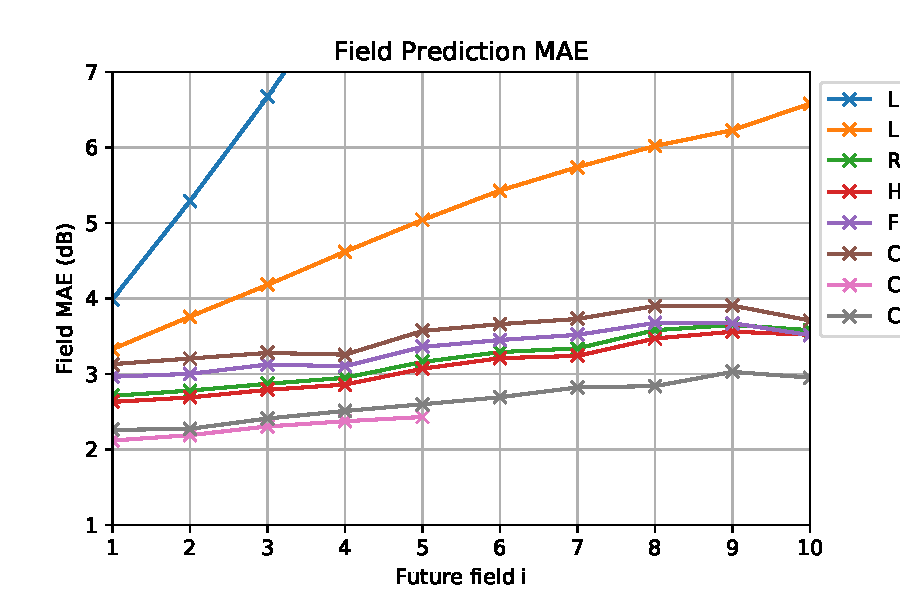
\includegraphics[width=0.8\textwidth]{field1.pdf}
		\caption{}
	\end{subfigure}
	\hfill
	\begin{subfigure}[b]{\textwidth}
		\centering
		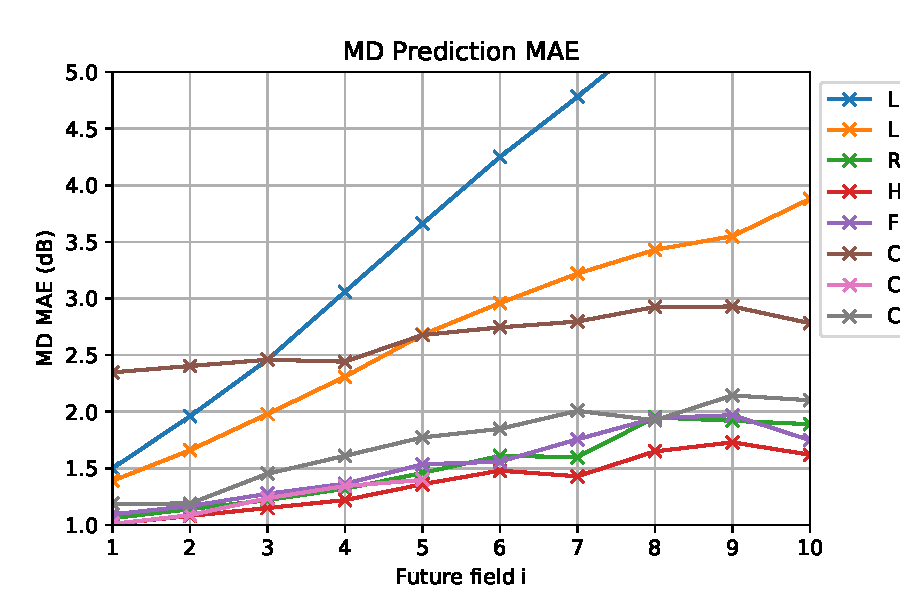
\includegraphics[width=0.8\textwidth]{md.pdf}
		\caption{}
	\end{subfigure}
	\caption[Field and \acs{MD} Prediction Results]{Field and \ac{MD} Prediction Results}
\end{figure}

\section{Discussion}



